%!TEX TS-program = xelatex
\documentclass[]{friggeri-cv}
%\usepackage{times}
\usepackage{afterpage}
\usepackage{hyperref}
\hypersetup{colorlinks=false,linkbordercolor=red,linkcolor=green,pdfborderstyle={/S/U/W 1}}

\usepackage{color}
\usepackage{xcolor}
\usepackage{smartdiagram}
\usepackage{fontspec}
% if you want to add fontawesome package
% you need to compile the tex file with LuaLaTeX
% References:
%   http://texdoc.net/texmf-dist/doc/latex/fontawesome/fontawesome.pdf
%   https://www.ctan.org/tex-archive/fonts/fontawesome?lang=en
\usepackage{fontawesome}
\usepackage{metalogo}
\usepackage{dtklogos}
\usepackage[utf8]{inputenc}
\usepackage{tikz}
\usetikzlibrary{mindmap,shadows}
\hypersetup{
    %pdftitle={resume},
    %pdfauthor={sergio_mazucato},
    %pdfsubject={},
    %pdfkeywords={},
    colorlinks=false,           % no lik border color
    allbordercolors=white       % white border color for all
}

\newfontfamily\myfont[Ligatures=TeX]{Times New Roman}

\smartdiagramset{
    bubble center node font = \footnotesize,
    bubble node font = \footnotesize,
    % specifies the minimum size of the bubble center node
    bubble center node size = 0.5cm,
    %  specifies the minimum size of the bubbles
    bubble node size = 0.5cm,
    % specifies which is the distance among the bubble center node and the other bubbles
    distance center/other bubbles = 0.3cm,
    % sets the distance from the text to the border of the bubble center node
    distance text center bubble = 0.5cm,
    % set center bubble color
    bubble center node color = pblue,
    % define the list of colors usable in the diagram
    set color list = {lightgray, materialcyan, orange, green, materialorange, materialteal, materialamber, materialindigo, materialgreen, materiallime},
    % sets the opacity at which the bubbles are shown
    bubble fill opacity = 0.6,
    % sets the opacity at which the bubble text is shown
    bubble text opacity = 0.5,
}

\addbibresource{bibliography.bib}
\RequirePackage{xcolor}
\definecolor{pblue}{HTML}{0395DE}

\begin{document}
\header{Sergio}{Mazucato}
      {Electrical Engineer}
      
% Fake text to add separator      
\fcolorbox{white}{gray}{\parbox{\dimexpr\textwidth-2\fboxsep-2\fboxrule}{%
.....
}}

% In the aside, each new line forces a line break
\begin{aside}
  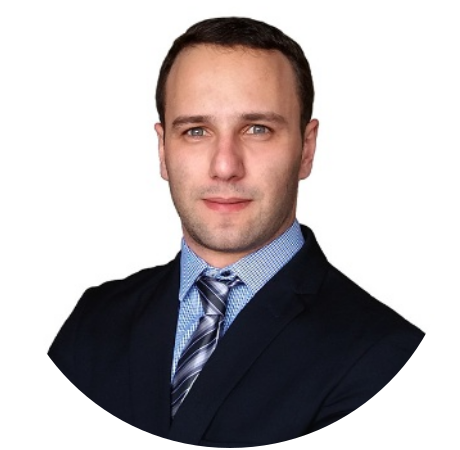
\includegraphics[scale=0.32]{img/linkedin_.png}
  \section{Contact}
    Ludwig-Pfau-Str.
    Heilbronn, 74074
    Deutschland
    ~
    +49 162 723 5023
    \href{mailto:sergiomazucato@gmail.com}{\textbf{sergiomazucato@}\\gmail.com}
    ~
  \section{Web References}
    \href{https://www.linkedin.com/in/sergiomazucato/}{LinkedIn}
    \href{https://www.xing.com/profile/Sergio_Mazucato}{Xing}
    \href{https://github.com/sergiomazucato}{GitHub}
    ~
  % use  \hspace{} or \vspace{} to change bubble size, if needed
	\section{Programming}
	    \textbf{Python}
\includegraphics[scale=0.38]{img/5bubbles.png}
	    \textbf{C}
\includegraphics[scale=0.38]{img/4bubbles.png}
	    \textbf{Matlab}
\includegraphics[scale=0.38]{img/5bubbles.png}
	    \textbf{Assembly}
\includegraphics[scale=0.38]{img/3bubbles.png}
	    ~
	\section{Languages}
	    \textbf{Portuguese}
\includegraphics[scale=0.40]{img/5stars.png}
	    \textbf{German}
\includegraphics[scale=0.40]{img/5stars.png}
	    \textbf{English}
\includegraphics[scale=0.40]{img/4stars.png}
	    \textbf{Italian}
\includegraphics[scale=0.40]{img/3stars.png}
	    ~
	\section{Places Lived}
		~
		
\includegraphics[scale=0.03]{img/brazil.png}    
\includegraphics[scale=0.03]{img/italy.png}   
\includegraphics[scale=0.03]{img/germany.png}
    	~
    \section{Appreciated Activities}
    	~
	    Problem solving 
\includegraphics[scale=0.40]{img/point.png}
	    Programming 
\includegraphics[scale=0.40]{img/point.png}
	    Electronics 
\includegraphics[scale=0.40]{img/point.png}
	    Math 
\includegraphics[scale=0.40]{img/point.png}
	    Playing Guitar 
\includegraphics[scale=0.40]{img/point.png}
	    Reading 
\includegraphics[scale=0.40]{img/point.png}
	    ~ 
\end{aside}
~
\section{Experience}
\begin{entrylist}

   \entry
    {10/19 - now}
    {Product Engineer}
    {\normalsize{Bosch Engineering (Abstatt)}}
    {Automotive function developer for the Inverters and DC-DC Converters of Bosch Engineering.
     \\}  
  
  \entry
    {10/18 -10/19}
    {Test Manager}
    {\normalsize{Bosch Engineering (Abstatt)}}
    {Test manager in charge of the Automotive ESP Projects of Bosch Engineering.
     \\}
  \entry
    {09/17 -10/18}
    {Technical Project Manager}
    {\normalsize{Thales (Stuttgart)}}
    {Technical Project Manager and Consultant for the Smartcards and software solutions of Thales (former Gemalto) in Stuttgart. 
     \\}
  \entry
    {09/16 - 08/17}
    {Technical Project Manager}
    {\normalsize{Thales (Sao Paulo)}}
    {Technical Project Manager for the Smartcards solutions of Thales (former Gemalto) in Sao Paulo.
    \\}
    \entry
    {08/15 - 08/16}
    {Project Engineer}
    {\normalsize{Thales (Sao Paulo)}}
    {Technical account leader of the Smartcards solutions and Data Processing related software of Thales (former Gemalto) in Sao Paulo. 
     \\}
    \entry
    {08/14 - 07/15}
    {Technical Consulting internship}
    {\normalsize{Thales (Sao Paulo)}}
    {Internship in the Project engineering department of Thales (former Gemalto) in Sao Paulo.
    \\}
    \entry
    {01/14 - 07/14}
    {Application Engineering internship}
    {\normalsize{Varixx electronics (Piracicaba)}}
    {Internship in the Application Engineering department of the Varixx in Piracicaba.
    \\}
\end{entrylist}
\section{Education}
\begin{entrylist}
  \entry
    {2016 - 2016}
    {Specialization in Project Management}
    {Fundacao Getulio Vargas (FGV)}
    {}
  \entry
    {2010 - 2015}
    {Bachelor's degree in Electrical Engineering}
    {Federal University of Parana}
    {cGPR: 3.28 - Rated as \textbf{best} student of the university at the National Exam for the Assessment of Student Performance.
    \\Honored as outstanding former stutendt.
    \\}
  \entry
    {2013}
    {ERASMUS}
    {FH-Zwickau}
    {IEEE Industrial Electronics Society \textbf{Award} in recognition for a paper presented at IECON2013 in Vienna.}
\end{entrylist}

%

%\begin{aside}
%~
%~
%~
%  \section{OS Preference}
%    \textbf{GNU/Linux}
\includegraphics[scale=0.40]{img/5stars.png}
%    \textbf{Unix}
\includegraphics[scale=0.40]{img/4stars.png}
%    \textbf{MacOS}
\includegraphics[scale=0.40]{img/2stars.png}
%    \textbf{Windows}
\includegraphics[scale=0.40]{img/1stars.png}
%    ~
%\end{aside}

\section{Publications}

\href{http://dx.doi.org/10.4018/ijncr.2014010101}{
\includegraphics[height=\fontcharht\font`\B]{img/igi_global_.png} Automatic Tuning of PSSs and PODs Using a Parallel Differential Evolution Algorithm. In: \textbf{2014 International Journal of Natural Computing Research}, v. 4, p. 1-16, 2014}.\\
\\
\href{http://dx.doi.org/10.1109/IECON.2013.6699462}{
\includegraphics[scale=0.11]{img/ieee.jpg} Parallel Simultaneous and Coordinated Tuning of PSSs Using Ant Colony Optimization. In: \textbf{2013 IEEE Industrial Electronics Society}, 2013 Vienna, Austria.}\\
\\
\href{http://dx.doi.org/10.1109/IECON.2013.6699436}{
\includegraphics[scale=0.11]{img/ieee.jpg} Combining Subpopulation Tables, Non-dominated Solutions and Strength Pareto of MOEAs to treat Service Restoration Problem in Large-Scale Distribution Systems. In: 2013 \textbf{IEEE Industrial Electronics Society}, 2013 Vienna, Austria.}\\
\\
\href{http://dx.doi.org/10.1109/PESGM.2012.6345340}{
\includegraphics[scale=0.11]{img/ieee.jpg} Simultaneous and coordinated tuning of PSSs and PODs using differential evolution. In: 2012 \textbf{IEEE Power \& Energy Society General Meeting}, 2012, San Diego. 2012 IEEE Power and Energy Society General Meeting.}\\
\\
\section{Complementary Info}

\begin{itemize}
	\item Linux basic knowledge (15+ years of personal use).
	\item Volunteer work for three years at two College projects: \textit{"Evolutive algorithms applied to corporeal exercises of people in rehab"} and \textit{"Local factors and regional potentialities of the city Cornelio Procopio"}.
	\item Teacher assistent during one year for \textit{Electrical Machinery} and \textit{Electricity and Magnetism}.
	\item This document was generated \footnote{compiled on \today} with Python and \myfont{\LaTeX} \footnote{\url{https://github.com/sergiomazucato/resume}}.\\
\end{itemize}



%\begin{flushleft}
%\emph{\today}%May 8th, 2016}
%\end{flushleft}

\end{document}
